\documentclass[tikz,border=20pt]{standalone}
\usepackage{amsmath,amssymb}
\usepackage{amsthm, amsfonts}
\usepackage{wasysym}
\usetikzlibrary{decorations.pathreplacing, calc, shadows, arrows.meta, positioning}

% Define the color palette
\definecolor{accent}{RGB}{20, 80, 180}       % Blue for Identity/Info/Structure
\definecolor{softaccent}{RGB}{230, 240, 255} 
\definecolor{parity}{RGB}{210, 80, 30}       % Orange for Transpose/Interaction
\definecolor{softparity}{RGB}{255, 235, 225} 
\definecolor{highlight}{RGB}{40, 140, 60}    % Green for Orthogonality
\definecolor{softhighlight}{RGB}{235, 250, 240}

\newcommand{\F}{\mathbb{F}}
\newcommand{\tp}{^{\mathsf T}}

\newcommand{\vect}[1]{\mathbf{#1}}
\newcommand{\code}{\mathcal{C}}

\begin{document}
%	\begin{tikzpicture}[
%		>=Stealth,
%		font=\sffamily,
%		% Styles for the matrix blocks
%		infoblock/.style={draw=accent, thick, fill=softaccent, rounded corners=2pt, drop shadow={opacity=0.15}},
%		parityblock/.style={draw=parity, thick, fill=softparity, rounded corners=2pt, drop shadow={opacity=0.15}},
%		% Styles for text and logic nodes
%		labeltext/.style={text=black!80},
%		mathsym/.style={font=\Large\bfseries, text=black!80},
%		logicnode/.style={fill=white, draw=black!30, thick, rounded corners=3pt, font=\small, align=center, inner sep=6pt, drop shadow={opacity=0.1}}
%		]
%		
%		% ==========================================
%		% TOP: GENERATOR MATRIX G
%		% ==========================================
%		% Dimensions: k rows. 
%		% I_k is a 3x3 square (Width 3, Height 3).
%		\draw[infoblock] (0, 3.5) rectangle (3.0, 6.5);
%		\node[mathsym, text=accent!80!black] at (1.5, 5.2) {$I_k$};
%		\node[text=accent!80!black, font=\scriptsize] at (1.5, 4.6) {$k \times k$};
%		
%		% Faint 1s for I_k
%		\draw[accent, very thin, dashed] (0.2, 6.3) -- (2.8, 3.7);
%		\node[text=accent, font=\tiny, fill=softaccent, inner sep=1pt] at (0.6, 5.9) {$1$};
%		\node[text=accent, font=\tiny, fill=softaccent, inner sep=1pt] at (2.4, 4.1) {$1$};
%		
%		% A is k x (n-k) (Width 2, Height 3)
%		\draw[parityblock] (3.2, 3.5) rectangle (5.2, 6.5);
%		\node[mathsym, text=parity!80!black] at (4.2, 5.2) {$A$};
%		\node[text=parity!80!black, font=\scriptsize] at (4.2, 4.6) {$k \times (n-k)$};
%		
%		% Labels for G
%		\draw[decorate, decoration={brace, amplitude=6pt}, thick] (0, 6.7) -- (5.2, 6.7);
%		\node[labeltext, font=\large\bfseries] at (2.6, 7.3) {Generator Matrix $G$};
%		
%		\draw[decorate, decoration={brace, amplitude=5pt, mirror}, thick, black!60] (-0.3, 6.5) -- (-0.3, 3.5);
%		\node[labeltext, font=\scriptsize\bfseries, text=black!60, rotate=90] at (-0.7, 5.0) {$k$ rows};
%		
%		
%		% ==========================================
%		% BOTTOM: PARITY-CHECK MATRIX H
%		% ==========================================
%		% Dimensions: n-k rows.
%		% -A^T is (n-k) x k. Since A was W=2, H=3, -A^T must be W=3, H=2.
%		% It aligns perfectly under I_k (Width 3).
%		\draw[parityblock] (0, 0) rectangle (3.0, 2.0);
%		\node[mathsym, text=parity!80!black] at (1.5, 1.2) {$-A^\tp$};
%		\node[text=parity!80!black, font=\scriptsize] at (1.5, 0.6) {$(n-k) \times k$};
%		
%		% I_{n-k} is (n-k) x (n-k) (Width 2, Height 2).
%		% It aligns perfectly under A (Width 2).
%		\draw[infoblock] (3.2, 0) rectangle (5.2, 2.0);
%		\node[mathsym, text=accent!80!black] at (4.2, 1.2) {$I_{n-k}$};
%		\node[text=accent!80!black, font=\scriptsize] at (4.2, 0.6) {$(n-k) \times (n-k)$};
%		
%		% Faint 1s for I_{n-k}
%		\draw[accent, very thin, dashed] (3.4, 1.8) -- (5.0, 0.2);
%		\node[text=accent, font=\tiny, fill=softaccent, inner sep=1pt] at (3.8, 1.4) {$1$};
%		\node[text=accent, font=\tiny, fill=softaccent, inner sep=1pt] at (4.6, 0.6) {$1$};
%		
%		% Labels for H
%		\draw[decorate, decoration={brace, amplitude=6pt, mirror}, thick] (0, -0.2) -- (5.2, -0.2);
%		\node[labeltext, font=\large\bfseries] at (2.6, -0.8) {Parity-Check Matrix $H$};
%		
%		\draw[decorate, decoration={brace, amplitude=5pt, mirror}, thick, black!60] (-0.3, 2.0) -- (-0.3, 0);
%		\node[labeltext, font=\scriptsize\bfseries, text=black!60, rotate=90] at (-0.7, 1.0) {$n-k$ rows};
%		
%		% Top/Bottom Column Braces
%		\draw[decorate, decoration={brace, amplitude=4pt}, thick, accent] (0, -1.4) -- (3.0, -1.4);
%		\node[labeltext, font=\scriptsize, text=accent] at (1.5, -1.8) {First $k$ columns};
%		
%		\draw[decorate, decoration={brace, amplitude=4pt}, thick, parity] (3.2, -1.4) -- (5.2, -1.4);
%		\node[labeltext, font=\scriptsize, text=parity] at (4.2, -1.8) {Last $n-k$ cols};
%		
%		% ==========================================
%		% TRANSFORMATION ARROW
%		% ==========================================
%		\draw[->, parity, thick, dashed] (4.2, 3.3) to[out=270, in=90, looseness=0.8] 
%		node[midway, logicnode, xshift=-15pt] {\color{parity!80!black}\textbf{Transpose \& Negate}} (1.5, 2.2);
%		
%		% ==========================================
%		% ORTHOGONALITY PROOF (RIGHT SIDE)
%		% ==========================================
%		\node[logicnode, inner sep=10pt, fill=softhighlight, draw=highlight, anchor=west] at (6.5, 3.25) {
%			\large\color{highlight!60!black}\textbf{Orthogonality Check: $GH^\tp = 0$}\\[2ex]
%			\normalsize\normalfont $G \cdot H^\tp = \begin{bmatrix} I_k & A \end{bmatrix} \cdot \begin{bmatrix} -A \\ I_{n-k} \end{bmatrix}$ \\[2ex]
%			$= I_k(-A) + A(I_{n-k})$ \\[1.5ex]
%			$= -A + A = \mathbf{0}$
%		};
%		
%	\end{tikzpicture}
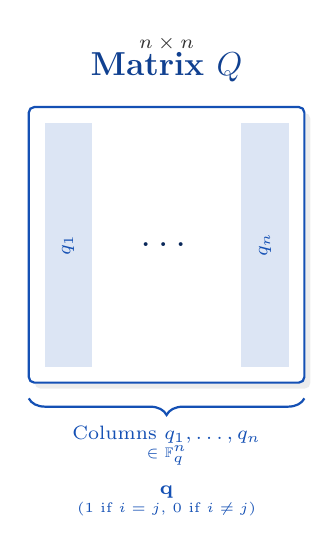
\begin{tikzpicture}[
	>=Stealth,
	font=\sffamily,
	% Styles for the matrix blocks
	infoblock/.style={draw=accent, thick, fill=white, rounded corners=2pt, drop shadow={opacity=0.15}},
	parityblock/.style={draw=parity, thick, fill=white, rounded corners=2pt, drop shadow={opacity=0.15}},
	% Styles for text and logic nodes
	labeltext/.style={text=black!80},
	mathsym/.style={font=\Large\bfseries, text=black!80},
	logicnode/.style={fill=white, draw=black!30, thick, rounded corners=3pt, font=\small, align=center, inner sep=6pt, drop shadow={opacity=0.1}},
	annotation/.style={font=\scriptsize\bfseries, text=black!70, align=left}
	]
	
	% ==========================================
	% MATRIX Q (LHS 1)
	% ==========================================
	% Accent block, columns represented conceptually
	\draw[infoblock] (0, 0) rectangle (3.5, 3.5);
	\node[labeltext, font=\large\bfseries, text=accent!80!black] at (1.75, 4.0) {Matrix $Q$};
	\node[labeltext, font=\scriptsize] at (1.75, 4.3) {$n \times n$};
	
	% Representing columns visually with braces and labels
	\draw[decorate, decoration={brace, amplitude=6pt, mirror}, thick, accent] (0, -0.2) -- (3.5, -0.2);
	\node[labeltext, font=\scriptsize, text=accent, align=center] at (1.75, -0.8) {Columns $q_1, \dots, q_n$\\[-0.5ex] \tiny $\in \F_q^n$};
	
	% Conceptual column highlights functionally
	\fill[accent!15] (0.2, 0.2) rectangle (0.8, 3.3);
	\node[accent, font=\scriptsize, rotate=90] at (0.5, 1.75) {$q_1$};
	\fill[accent!15] (2.7, 0.2) rectangle (3.3, 3.3);
	\node[accent, font=\scriptsize, rotate=90] at (3.0, 1.75) {$q_n$};
	\node[mathsym, font=\Large, text=accent!50!black] at (1.75, 1.75) {$\dots$};
	
	% Labels for orthogonality of cols
	\node[labeltext, text=accent, font=\scriptsize, align=center] at (1.75, -1.5) {
		$\vect{q}$%$\vect{q}_i^\tp \vect{q}_j = \delta_{ij}}$
	\\[-0.5ex]
	\tiny ($1$ if $i=j$, $0$ if $i\neq j$)};
	
%	% Multiplication sign
%	\node[mathsym] at (4.25, 1.75) {$\times$};
%	
%	% ==========================================
%	% MATRIX Q^T (LHS 2)
%	% ==========================================
%	% Parity block, rows represented conceptually (columns of Q transpose)
%	\draw[parityblock] (5.0, 0) rectangle (8.5, 3.5);
%	\node[labeltext, font=\large\bfseries, text=parity!80!black] at (6.75, 4.0) {Matrix $Q^\tp$};
%	\node[labeltext, font=\scriptsize] at (6.75, 4.3) {$n \times n$};
%	
%	% Representing rows visually with braces and labels
%	\draw[decorate, decoration={brace, amplitude=6pt}, thick, parity] (4.8, 0) -- (4.8, 3.5);
%	\node[labeltext, font=\scriptsize, text=parity, rotate=90, align=center] at (4.2, 1.75) {Rows $q_1^\tp, \dots, q_n^\tp$\\[-0.5ex] \tiny $\in (\F_q^n)^\tp$};
%	
%	% Conceptual row highlights functionally
%	\fill[parity!15] (5.2, 2.7) rectangle (8.3, 3.3);
%	\node[parity, font=\scriptsize] at (6.75, 3.0) {$q_1^\tp$};
%	\fill[parity!15] (5.2, 0.2) rectangle (8.3, 0.8);
%	\node[parity, font=\scriptsize] at (6.75, 0.5) {$q_n^\tp$};
%	\node[mathsym, font=\Large, text=parity!50!black] at (6.75, 1.75) {$\vdots$};
%	
%	% Labels for transpose property
%	\node[labeltext, text=parity, font=\scriptsize, align=center] at (6.75, -0.6) {Rows of $Q^\tp$ are\\[-0.5ex] \tiny columns of $Q$ transpose};
%	
%	% Equals sign
%	\node[mathsym] at (9.25, 1.75) {$=$};
%	
%	% ==========================================
%	% PRODUCT MATRIX (I)
%	% ==========================================
%	% Accent block, identity matrix
%	\draw[infoblock] (10.0, 0) rectangle (13.5, 3.5);
%	\node[labeltext, font=\large\bfseries, text=accent!80!black] at (11.75, 4.0) {Product $Q^\tp Q$};
%	\node[labeltext, font=\scriptsize] at (11.75, 4.3) {$n \times n$};
%	
%	% Representing I matrix content
%	\node[mathsym, text=accent!80!black] at (10.3, 3.2) {$1$};
%	\node[mathsym, text=black!50] at (13.2, 3.2) {$0$};
%	\node[mathsym, text=black!50] at (10.3, 0.3) {$0$};
%	\node[mathsym, text=accent!80!black] at (13.2, 0.3) {$1$};
%	
%	\node[font=\Large, text=black!30] at (11.75, 2.6) {$0$};
%	\node[font=\Large, text=black!30] at (11.75, 0.9) {$0$};
%	\node[font=\Large, text=black!30, rotate=90] at (10.8, 1.75) {$0$};
%	\node[font=\Large, text=black!30, rotate=90] at (12.7, 1.75) {$0$};
%	
%	% Highlight diagonal functionally
%	\fill[accent!15, opacity=0.5] (10.15, 3.05) rectangle (10.45, 3.35);
%	\fill[accent!15, opacity=0.5] (13.05, 0.15) rectangle (13.35, 0.45);
%	\draw[accent, very thin, dashed] (10.2, 3.2) -- (13.3, 0.4);
%	\node[text=accent, font=\tiny, fill=softaccent, inner sep=1pt] at (10.6, 2.8) {$1$};
%	\node[text=accent, font=\tiny, fill=softaccent, inner sep=1pt] at (12.9, 0.7) {$1$};
%	
%	% Conceptual element representation showing dot product visually
%	\fill[softparity] (11.0, 1.4) rectangle (12.5, 2.1);
%	\node[font=\small, text=black!80, align=center] at (11.75, 1.75) {$\vect{q_i^\tp} \vect{q_j}$};
%	\draw[decorate, decoration={brace, amplitude=4pt, mirror}, parity] (11.0, 1.3) -- (12.5, 1.3);
%	\node[labeltext, font=\scriptsize, text=parity] at (11.75, 1.0) {\tiny Row $i$ from $Q^\tp$\\[-0.5ex] \tiny $\vect{q_i}$ (col i of Q)};
%	\draw[decorate, decoration={brace, amplitude=4pt, mirror}, accent] (13.6, 1.4) -- (13.6, 2.1);
%	\node[labeltext, font=\scriptsize, text=accent, align=center, rotate=-90] at (14.2, 1.75) {\tiny Col $j$ from $Q$\\[-0.5ex] \tiny $\vect{q_j}$};
%	
%	% Label for Identity properties
%	\node[labeltext, font=\small\bfseries, text=accent, align=center] at (11.75, -0.8) {Identity Matrix $I_n$\\[-0.5ex]\tiny ($q_i^\tp q_i=1$, $q_i^\tp q_j=0$ for $i\neq j$)};
	
\end{tikzpicture}
\end{document}